\documentclass[12pt,a4paper]{article}

% ─── Page Layout ───────────────────────────────────────────────────────────────
\usepackage[a4paper, margin=0.8in, headheight=14pt]{geometry}

% ─── Fonts (XeLaTeX) ───────────────────────────────────────────────────────────
\usepackage{fontspec}
\usepackage{unicode-math}
\setmainfont{TeX Gyre Pagella}
\setmonofont[Scale=0.88]{TeX Gyre Cursor}
\setmathfont{Latin Modern Math}

% ─── Packages ──────────────────────────────────────────────────────────────────
\usepackage{xcolor}
\usepackage{colortbl}
\usepackage{titlesec}
\usepackage{enumitem}
\usepackage{tabularx}
\usepackage{booktabs}
\usepackage{array}
\usepackage{amsmath}
\usepackage{tikz}
\usetikzlibrary{shapes.geometric, arrows.meta, positioning, calc, fit, decorations.pathreplacing, patterns, backgrounds}
\usepackage{tcolorbox}
\tcbuselibrary{skins, breakable}
\usepackage{hyperref}
\usepackage{fancyhdr}
\usepackage{graphicx}
\usepackage{microtype}
\hyphenpenalty=10000
\exhyphenpenalty=10000
\sloppy
\usepackage{caption}
\usepackage{setspace}
\usepackage{multirow}
\usepackage{tocloft}

% ─── Q&A helper ────────────────────────────────────────────────────────────────
\newcommand{\Q}[1]{\textbf{#1}\par\noindent\ignorespaces}

% ─── Colour Palette ────────────────────────────────────────────────────────────
\definecolor{myred}{RGB}{196,30,58}
\definecolor{mydark}{RGB}{30,30,50}
\definecolor{mygreen}{RGB}{14,120,80}
\definecolor{myteal}{RGB}{0,130,140}
\definecolor{myamber}{RGB}{180,100,0}
\definecolor{mypurple}{RGB}{100,30,160}
\definecolor{mygray}{RGB}{246,247,249}
\definecolor{mgframe}{RGB}{180,185,200}
\definecolor{watermark}{RGB}{145,150,170}
\definecolor{hdrred}{RGB}{250,232,235}
\definecolor{hdrgreen}{RGB}{220,244,233}
\definecolor{hdrteal}{RGB}{220,242,244}
\definecolor{hdramber}{RGB}{253,242,215}
\definecolor{hdrpurple}{RGB}{238,228,255}
\definecolor{hdrgray}{RGB}{238,240,245}
\definecolor{rowalt}{RGB}{250,251,253}

% ─── Section Formatting ────────────────────────────────────────────────────────
\titleformat{\section}{\large\bfseries\color{myred}}{\thesection.}{0.5em}{}[\vspace{1pt}{\color{myred}\rule{\linewidth}{0.8pt}}]
\titleformat{\subsection}{\normalsize\bfseries\color{myteal}}{\thesubsection}{0.5em}{}
\titlespacing*{\section}{0pt}{18pt}{7pt}
\titlespacing*{\subsection}{0pt}{11pt}{4pt}

% ─── Paragraph ─────────────────────────────────────────────────────────────────
\setlength{\parindent}{0pt}
\setlength{\parskip}{4pt}

% ─── TOC Styling ───────────────────────────────────────────────────────────────
\renewcommand{\cfttoctitlefont}{\large\bfseries\color{myred}}
\renewcommand{\cftaftertoctitle}{\par\noindent{\color{myred}\rule{\linewidth}{0.8pt}}}
\setlength{\cftbeforetoctitleskip}{0pt}
\setlength{\cftaftertoctitleskip}{6pt}
\renewcommand{\cftsecfont}{\normalsize\bfseries\color{mydark}}
\renewcommand{\cftsecpagefont}{\normalsize\bfseries\color{mydark}}
\renewcommand{\cftsecleader}{\cftdotfill{\cftdotsep}}
\setlength{\cftbeforesecskip}{7pt}
\renewcommand{\cftsubsecfont}{\small\color{mydark}}
\renewcommand{\cftsubsecpagefont}{\small\color{mydark}}
\setlength{\cftbeforesubsecskip}{3pt}
\setlength{\cftsubsecindent}{1.4em}

% ─── Table helpers ─────────────────────────────────────────────────────────────
\renewcommand{\arraystretch}{1.45}
\setlength{\tabcolsep}{6pt}
\arrayrulecolor{mydark}
\newcolumntype{B}[1]{>{\small\bfseries\raggedright\arraybackslash}m{#1}}
\newcolumntype{Y}{>{\small\raggedright\arraybackslash}X}
\renewcommand{\tabularxcolumn}[1]{m{#1}}

% ─── Header / Footer ───────────────────────────────────────────────────────────
\pagestyle{fancy}
\fancyhf{}
\fancyhead[L]{\small\color{myred}\textbf{OE-EC803B}\;\color{mydark}--- Big Data Analysis}
\fancyhead[R]{\small\color{myteal}\textbf{Module 0 Notes}}
\fancyfoot[C]{\small\color{mydark}\thepage}
\fancyfoot[R]{\small\color{watermark}\textit{\copyright\ Biraj Sarkar}}
\renewcommand{\headrulewidth}{0.5pt}
\renewcommand{\footrulewidth}{0.3pt}

% ─── Hyperref ──────────────────────────────────────────────────────────────────
\hypersetup{colorlinks=true, linkcolor=myteal, urlcolor=myteal,
  pdfauthor={Biraj Sarkar}, pdftitle={OE-EC803B --- Module 0 Notes}}

% ─── tcolorbox styles ──────────────────────────────────────────────────────────
\tcbset{
  tikzbox/.style={colback=mygray, colframe=mgframe, boxrule=0.6pt, arc=4pt,
    left=8pt, right=8pt, top=6pt, bottom=6pt,
    colbacktitle=mgframe, coltitle=mydark, fonttitle=\small\bfseries, unbreakable},
  defbox/.style={colback=hdrgreen, colframe=mygreen, boxrule=0.8pt, arc=4pt,
    left=9pt, right=9pt, top=6pt, bottom=6pt,
    colbacktitle=mygreen, coltitle=white, fonttitle=\small\bfseries},
  formulabox/.style={colback=hdrteal, colframe=myteal, boxrule=0.8pt, arc=4pt,
    left=9pt, right=9pt, top=7pt, bottom=7pt,
    colbacktitle=myteal, coltitle=white, fonttitle=\small\bfseries},
  examplebox/.style={colback=hdramber, colframe=myamber, boxrule=0.8pt, arc=4pt,
    left=9pt, right=9pt, top=6pt, bottom=6pt,
    colbacktitle=myamber, coltitle=white, fonttitle=\small\bfseries},
  masonbox/.style={colback=hdrpurple, colframe=mypurple, boxrule=0.8pt, arc=4pt,
    left=9pt, right=9pt, top=6pt, bottom=6pt,
    colbacktitle=mypurple, coltitle=white, fonttitle=\small\bfseries},
  exambox/.style={colback=hdrpurple, colframe=mypurple, boxrule=1pt, arc=5pt,
    left=10pt, right=10pt, top=8pt, bottom=8pt,
    colbacktitle=mypurple, coltitle=white, fonttitle=\bfseries,
    breakable, title after break={\textbf{Frequently Asked / Viva Questions (contd.)}}}
}
\tcbset{breakable}

% ─── TikZ styles ───────────────────────────────────────────────────────────────
\tikzset{
  block/.style={rectangle, draw=myteal, fill=hdrteal,
    text width=2.2cm, align=center, minimum height=0.9cm,
    font=\small, rounded corners=3pt, line width=0.7pt},
  redblock/.style={rectangle, draw=myred, fill=hdrred,
    text width=2.2cm, align=center, minimum height=0.9cm,
    font=\small, rounded corners=3pt, line width=0.7pt},
  arrow/.style={-Stealth, thick, color=mydark},
  redarrow/.style={-Stealth, thick, color=myred},
  line/.style={thick, color=mydark}
}

\begin{document}

% ═══════════════════════════════════════════════════════════════════════════════
% TITLE BLOCK
% ═══════════════════════════════════════════════════════════════════════════════
\begin{center}
  \hfill \textit{Exam-Ready Short Notes} \\
  \vspace{6pt}
  {\LARGE\bfseries\color{myred} OE-EC803B --- Big Data Analysis}\\[5pt]
  {\normalsize\color{mydark} Semester VIII \quad$\bullet$\quad 3L:0T:0P \quad$\bullet$\quad 3 Credits}\\[3pt]
  {\normalsize\color{myteal}\textbf{Module 0: Pre-requisite Computer Science Fundamentals}}\\[3pt]
  {\small\color{mydark} CGEC \;$|$\; B.Tech ECE (2023--27) \;$|$\; \textit{Biraj Sarkar}}
\end{center}
\vspace{2pt}
\noindent{\color{myred}\rule{\linewidth}{1.5pt}}
\vspace{2pt}

\hypersetup{linkcolor=mydark}
\tableofcontents
\hypersetup{linkcolor=myteal}
\newpage

% ===============================================================================
\section{Java Programming \& OOP Foundations}
% ===============================================================================

Distributed frameworks in the Hadoop Ecosystem are heavily built on Java. A strong grasp of Java's runtime environment and Object-Oriented Programming (OOP) paradigms is essential to understand HDFS mechanics and MapReduce workflows.

\begin{tcolorbox}[defbox, title={Java Virtual Machine (JVM)}]
  The \textbf{Java Virtual Machine (JVM)} is an abstract computing machine that provides a runtime environment in which Java bytecode can be executed. It acts as an engine that drives the execution of Java code, converting bytecode to machine-specific instructions and managing system memory.
\end{tcolorbox}

\subsection{Object-Oriented Programming (OOP) Principles}
Java uses four primary OOP pillars which map directly to distributed programming:
\begin{itemize}[leftmargin=*, itemsep=3pt]
  \item \textbf{Encapsulation:} Bundling fields and methods within a single class and restricting direct access (using access modifiers like `private`, `protected`, `public`) to protect the internal state of objects.
  \item \textbf{Inheritance:} Allowing a class (subclass) to inherit fields and methods from another class (superclass). In Hadoop, custom mappers and reducers inherit from base API classes.
  \item \textbf{Polymorphism:} The ability of an object to take on many forms. Used in Hadoop when custom serialized types implement interface contracts (e.g., overriding the `write()` and `readFields()` methods of the `Writable` interface).
  \item \textbf{Abstraction:} Hiding implementation details and showing only functional interfaces using `abstract` classes and `interfaces`.
\end{itemize}

\subsection{Java Collections Framework}
In MapReduce, intermediate values are held in collection data structures. The framework provides three primary categories of collections:

\par\vspace{6pt}\noindent
{\renewcommand{\arraystretch}{1.4}%
\begin{tabularx}{\linewidth}{|B{3.0cm}|Y|B{3.2cm}|Y|}
\hline
\textbf{Collection} & \textbf{Key Characteristics} & \textbf{Underlying Structure} & \textbf{Hadoop Use Case} \\
\hline
`ArrayList` & Ordered, indexable list. Allows duplicates. Resizes dynamically. & Resizable Array & Gathering list of values associated with a single key in Reducer. \\
\hline
`HashSet` & Unordered collection. No duplicates allowed. & Hash Table & Filtering out duplicate records or keys during processing. \\
\hline
`HashMap` & Key-value pairs storage. Unique keys. Fast search. & Hash Table + Linked List & Local in-memory caching and Map-Side Joins. \\
\hline
\end{tabularx}}

\subsection{JVM Memory Management}
The JVM splits its runtime memory into distinct regions. Understanding this is key to debugging Out-Of-Memory (OOM) errors in Hadoop:
\begin{itemize}[leftmargin=*, itemsep=3pt]
  \item \textbf{Stack Memory:} Stores local variables and method execution frames. Allocation and deallocation are managed automatically.
  \item \textbf{Heap Memory:} Stores all objects instantiated via the `new` keyword. Managed by the JVM \textbf{Garbage Collector (GC)}. If MapReduce buffers grow too large, Heap memory exhaustion triggers a JVM crash.
\end{itemize}

\begin{tcolorbox}[tikzbox, title={JVM Heap and Stack Memory Structure}]
\centering
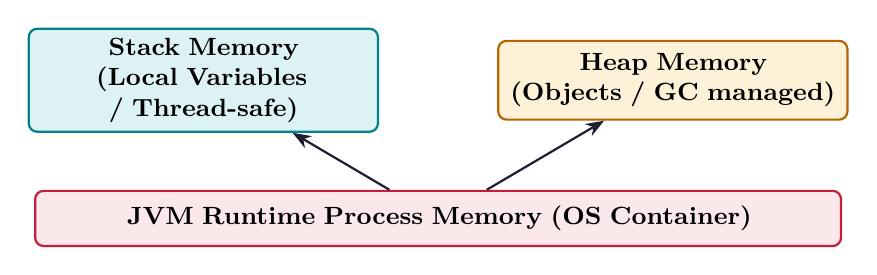
\begin{tikzpicture}[node distance=1.2cm and 1.5cm,
  mblock/.style={rectangle, draw=myteal, fill=hdrteal, text width=4.2cm, align=center, minimum height=1.0cm, font=\small\bfseries, rounded corners=3pt, line width=0.8pt},
  gblock/.style={rectangle, draw=myamber, fill=hdramber, text width=4.2cm, align=center, minimum height=1.0cm, font=\small\bfseries, rounded corners=3pt, line width=0.8pt},
  rblock/.style={rectangle, draw=myred, fill=hdrred, text width=10.0cm, align=center, minimum height=0.7cm, font=\small\bfseries, rounded corners=3pt, line width=0.8pt}]

  % Stack Nodes
  \node[mblock] (stack) {Stack Memory\\(Local Variables / Thread-safe)};
  
  % Heap Nodes
  \node[gblock, right=of stack] (heap) {Heap Memory\\(Objects / GC managed)};

  % Shared System Node
  \node[rblock, below=0.8cm of $(stack.south)!0.5!(heap.south)$] (jvm) {JVM Runtime Process Memory (OS Container)};

  % Connections
  \draw[arrow] (jvm) -- (stack);
  \draw[arrow] (jvm) -- (heap);
  
\end{tikzpicture}
\end{tcolorbox}

% ===============================================================================
\section{Structured Query Language (SQL) \& Relational Algebra}
% ===============================================================================

Data warehouse systems like Apache Hive use HiveQL, which is a dialect of SQL. Distributed querying translates SQL declarations into computational graphs.

\begin{tcolorbox}[defbox, title={Relational Databases vs. Hadoop Queries}]
  Traditional databases use \textbf{Schema-on-Write}, validating data constraints during insertion. SQL engines on Hadoop (like Hive and Big SQL) use \textbf{Schema-on-Read}, overlaying structure on top of raw file streams (e.g., text, CSV, ORC) at query execution time.
\end{tcolorbox}

\subsection{Logical Execution Order of an SQL Query}
While SQL queries are written starting with the `SELECT` clause, the SQL compiler executes operations in a different logical sequence:

\begin{tcolorbox}[formulabox, title={Logical SQL Execution Order}]
  $$\text{FROM} \longrightarrow \text{JOIN} \longrightarrow \text{WHERE} \longrightarrow \text{GROUP BY} \longrightarrow \text{HAVING} \longrightarrow \text{SELECT} \longrightarrow \text{ORDER BY}$$
  \begin{itemize}[leftmargin=*, noitemsep]
    \item \textbf{FROM/JOIN:} Identifies target datasets and links them.
    \item \textbf{WHERE:} Filters rows based on non-aggregated predicates.
    \item \textbf{GROUP BY:} Groups rows based on key values.
    \item \textbf{HAVING:} Filters groups using aggregate functions (e.g., `HAVING count(*) > 5`).
    \item \textbf{SELECT:} Projects fields and calculates functions.
    \item \textbf{ORDER BY:} Sorts output (very expensive in distributed systems as it forces global sorting).
  \end{itemize}
\end{tcolorbox}

\subsection{SQL Joins}
Joins are fundamental operations that merge datasets horizontally on a matching key column:
\begin{itemize}[leftmargin=*, itemsep=3pt]
  \item \textbf{Inner Join:} Returns records that have matching values in both tables.
  \item \textbf{Left (Outer) Join:} Returns all records from the left table, and matched records from the right table. Fill with `NULL` on the right side if no match.
  \item \textbf{Right (Outer) Join:} Returns all records from the right table, and matched records from the left table.
  \item \textbf{Full (Outer) Join:} Returns all records when there is a match in either left or right table.
\end{itemize}

\begin{tcolorbox}[tikzbox, title={SQL Joins Visual Representation}]
\centering
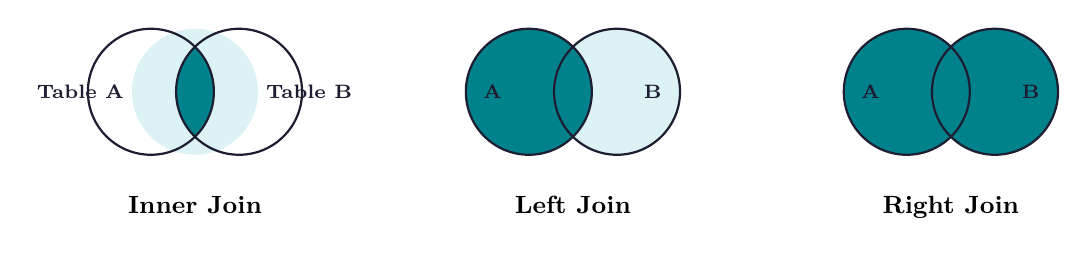
\begin{tikzpicture}[scale=0.8]
  % Set styles
  \tikzset{set/.style={circle, minimum size=2.8cm, fill opacity=0.4, line width=0.8pt}}

  % Inner Join Group
  \begin{scope}[shift={(0,0)}]
    \fill[hdrteal] (0.7,0) circle (1.0cm);
    \begin{scope}
      \clip (0,0) circle (1.0cm);
      \fill[myteal] (1.4,0) circle (1.0cm);
    \end{scope}
    \draw[line] (0,0) circle (1.0cm) node[left=6pt, font=\scriptsize\bfseries] {Table A};
    \draw[line] (1.4,0) circle (1.0cm) node[right=6pt, font=\scriptsize\bfseries] {Table B};
    \node[below=1.2cm] at (0.7,0) {\small\bfseries Inner Join};
  \end{scope}

  % Left Join Group
  \begin{scope}[shift={(6.0,0)}]
    \fill[myteal] (0,0) circle (1.0cm);
    \fill[hdrteal] (1.4,0) circle (1.0cm);
    \begin{scope}
      \clip (0,0) circle (1.0cm);
      \fill[myteal] (1.4,0) circle (1.0cm);
    \end{scope}
    \draw[line] (0,0) circle (1.0cm) node[left=6pt, font=\scriptsize\bfseries] {A};
    \draw[line] (1.4,0) circle (1.0cm) node[right=6pt, font=\scriptsize\bfseries] {B};
    \node[below=1.2cm] at (0.7,0) {\small\bfseries Left Join};
  \end{scope}

  % Right Join Group
  \begin{scope}[shift={(12.0,0)}]
    \fill[hdrteal] (0,0) circle (1.0cm);
    \fill[myteal] (1.4,0) circle (1.0cm);
    \begin{scope}
      \clip (0,0) circle (1.0cm);
      \fill[myteal] (0,0) circle (1.0cm);
    \end{scope}
    \draw[line] (0,0) circle (1.0cm) node[left=6pt, font=\scriptsize\bfseries] {A};
    \draw[line] (1.4,0) circle (1.0cm) node[right=6pt, font=\scriptsize\bfseries] {B};
    \node[below=1.2cm] at (0.7,0) {\small\bfseries Right Join};
  \end{scope}
\end{tikzpicture}
\end{tcolorbox}

\subsection{Subqueries and Common Table Expressions (CTEs)}
\begin{itemize}[leftmargin=*, itemsep=3pt]
  \item \textbf{Subquery:} A query nested inside another SQL statement. It can return scalar values, single columns, or tables (e.g., `SELECT * FROM emp WHERE salary > (SELECT AVG(salary) FROM emp)`).
  \item \textbf{Common Table Expression (CTE):} A temporary named result set defined using the `WITH` keyword, which improves readability compared to nested subqueries:
\end{itemize}

\begin{tcolorbox}[examplebox, title={Common Table Expression (CTE) Syntax}]
  \begin{spacing}{0.95}
  \begin{verbatim}
  WITH DeptAvgSalary AS (
      SELECT dept_id, AVG(salary) AS avg_sal
      FROM employees
      GROUP BY dept_id
  )
  SELECT e.name, e.salary, d.avg_sal
  FROM employees e
  JOIN DeptAvgSalary d ON e.dept_id = d.dept_id;
  \end{verbatim}
  \end{spacing}
\end{tcolorbox}

% ===============================================================================
\section{Linux Command Line \& Unix Text Processing}
% ===============================================================================

Hadoop CLI commands mimic standard Linux file system operations. Exposure to Unix text processing tools is essential for filtering, parsing, and verifying datasets before importing them.

\begin{tcolorbox}[defbox, title={Unix Streams}]
  Unix systems model communications via three standard input/output channels (streams):
  \begin{itemize}[leftmargin=*, noitemsep]
    \item \textbf{stdin (0):} Standard Input stream (default: keyboard).
    \item \textbf{stdout (1):} Standard Output stream (default: terminal screen).
    \item \textbf{stderr (2):} Standard Error stream (default: terminal screen).
  \end{itemize}
\end{tcolorbox}

\subsection{Core File Manipulation Commands}
\begin{itemize}[leftmargin=*, itemsep=3pt]
  \item `cd <dir>`: Change current working directory.
  \item `ls -la`: List directory contents showing file size, permissions, and hidden files.
  \item `mkdir -p <path>`: Create directories recursively without throwing errors if they exist.
  \item `cp -r <src> <dest>`: Copy files and directories recursively.
  \item `mv <src> <dest>`: Move or rename files.
  \item `rm -rf <path>`: Recursively force delete files or directories.
  \item `chmod 755 <file>`: Modify file read-write-execute permissions (rwxr-xr-x).
\end{itemize}

\subsection{Redirections and Pipelines}
Commands can output data to files or other commands instead of printing to the terminal:
\begin{itemize}[leftmargin=*, itemsep=3pt]
  \item \textbf{Redirections:} Redirect outputs or inputs to files.
        \begin{itemize}[leftmargin=*, noitemsep]
          \item `>`: Redirects `stdout` to a file (overwriting existing content).
          \item `>>`: Appends `stdout` to a file.
          \item `2>`: Redirects `stderr` to a file.
        \end{itemize}
  \item \textbf{Pipes (`|`):} Passes the `stdout` of one command as the `stdin` of the next command.
\end{itemize}

\begin{tcolorbox}[tikzbox, title={Pipeline Data Flow}]
\centering
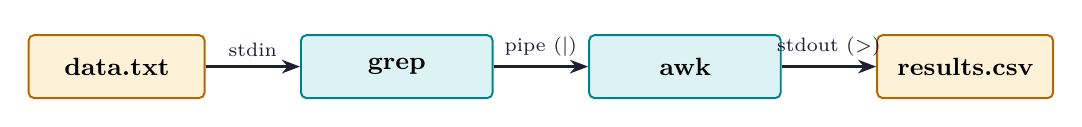
\begin{tikzpicture}[node distance=1.1cm and 1.2cm,
  cblock/.style={rectangle, draw=myteal, fill=hdrteal, text width=2.2cm, align=center, minimum height=0.8cm, font=\small\bfseries, rounded corners=2pt, line width=0.7pt},
  fblock/.style={rectangle, draw=myamber, fill=hdramber, text width=2.0cm, align=center, minimum height=0.8cm, font=\small\bfseries, rounded corners=2pt, line width=0.7pt}]

  % Nodes
  \node[fblock] (file) {data.txt};
  \node[cblock, right=of file] (c1) {grep};
  \node[cblock, right=of c1] (c2) {awk};
  \node[fblock, right=of c2] (out) {results.csv};

  % Paths
  \draw[arrow] (file) -- node[above, font=\scriptsize] {stdin} (c1);
  \draw[arrow] (c1) -- node[above, font=\scriptsize] {pipe (|)} (c2);
  \draw[arrow] (c2) -- node[above, font=\scriptsize] {stdout (>)} (out);

\end{tikzpicture}
\end{tcolorbox}

\subsection{Unix Text Processing Tools}
Hadoop Streaming allows using Unix programs as mappers and reducers. The core tools are:
\begin{itemize}[leftmargin=*, itemsep=3pt]
  \item `cat`: Concatenates and displays file contents.
  \item `grep <pattern>`: Searches for regular expression pattern matches within files.
  \item \texttt{awk}: A pattern scanning and processing language. Heavily used to extract columns (e.g., \texttt{awk '\{print \$2\}'} extracts the second space-separated field).
  \item `sed`: A stream editor for parsing and transforming text (e.g., substitute strings).
  \item `sort`: Sorts lines of text files alphabetically or numerically.
  \item `uniq`: Discards duplicate adjacent lines. Needs data to be pre-sorted.
\end{itemize}

\begin{tcolorbox}[examplebox, title={Common UNIX Text Processing Pipeline}]
  To find the top 5 most frequent error types from a log file:
  \begin{spacing}{0.95}
  \begin{verbatim}
  cat server.log | grep "ERROR" | awk '{print $5}' | sort | uniq -c | sort -nr | head -n 5
  \end{verbatim}
  \end{spacing}
  \textbf{Explanation:} 
  Step 1: Print file $\longrightarrow$ Step 2: Filter lines containing "ERROR" $\longrightarrow$ Step 3: Extract the fifth column $\longrightarrow$ Step 4: Sort columns $\longrightarrow$ Step 5: Count occurrences of unique elements $\longrightarrow$ Step 6: Sort counts numerically in descending order $\longrightarrow$ Step 7: Print top 5 lines.
\end{tcolorbox}

\newpage

% ═══════════════════════════════════════════════════════════════════════════════
% QUICK REVISION PAGE
% ═══════════════════════════════════════════════════════════════════════════════
\begin{center}
  {\large\bfseries\color{myred} Quick Revision --- Module 0}\\[3pt]
  {\small\color{mydark} Java Collections, SQL Queries \& Unix Pipelines $|$ OE-EC803B}
\end{center}
\noindent{\color{myred}\rule{\linewidth}{1.2pt}}
\vspace{8pt}

\begin{tcolorbox}[defbox, title={\textbf{One-Line Definitions}}]
\begin{itemize}[leftmargin=*, itemsep=3pt, topsep=0pt]
  \item \textbf{Polymorphism:} The OOP capability to invoke object-specific methods via interface abstractions.
  \item \textbf{Schema-on-Read:} A data schema validation approach where structure is applied only when reading files.
  \item \textbf{Common Table Expression (CTE):} A temporary named result set defined locally within an SQL query block.
  \item \textbf{Unix Pipe:} A mechanism that directs the standard output of one command to the standard input of another.
  \item \textbf{Garbage Collector (GC):} A background JVM process that automatically reclaims memory by deleting unreferenced objects.
\end{itemize}
\end{tcolorbox}

\vspace{6pt}

\begin{tcolorbox}[exambox, title={\textbf{Frequently Asked / Viva Questions}}]
\begin{enumerate}[leftmargin=*, topsep=0pt, label=\textbf{Q\arabic*.}, itemsep=5pt]
  \item \Q{Why is Java memory management critical in Hadoop MapReduce jobs?}
        Custom mapper and reducer code instantiates objects inside JVM heap containers. If collections (like lists or hash maps) grow indefinitely without boundary checks, JVM Heap runs out of memory, leading to job failure.
        
  \item \Q{Compare SQL's WHERE and HAVING clauses.}
        The `WHERE` clause filters individual rows before grouping operations occur. The `HAVING` clause filters aggregated groups after the `GROUP BY` clause has been processed.
        
  \item \Q{Explain the utility of SQL Subqueries vs. CTEs.}
        Subqueries are nested expressions that can make queries complex and hard to read. Common Table Expressions (CTEs) define clear, modular virtual tables using `WITH`, facilitating compiler optimization and improving readability.
        
  \item \Q{What does the command ``chmod 755 script.sh'' accomplish?}
        It sets file permissions: Owner receives full permissions (Read=4, Write=2, Execute=1 $\to$ 7). Group and Others receive Read and Execute permissions (Read=4, Execute=1 $\to$ 5).
        
  \item \Q{Why must ``uniq'' be preceded by a ``sort'' command in Unix pipelines?}
        The `uniq` command only matches and filters out adjacent duplicate lines. If duplicate records are scattered, `uniq` will miss them. Pre-sorting groups duplicate lines together.
        
  \item \Q{What is the difference between ``>'' and ``>>'' in Unix Shell?}
        `>` redirects standard output to a file, overwriting the file's current contents. `>>` redirects output to a file, appending the output at the end of the file.
        
  \item \Q{Describe the JVM Stack vs. Heap memory allocations.}
        Stack allocation is temporary, storing thread execution states and primitive local variables. Heap stores dynamic class objects that require garbage collection.
        
  \item \Q{What is the time complexity of looking up a key in a HashMap?}
        On average, `HashMap` lookup has $O(1)$ constant time complexity. In the worst case (with hash collisions), it defaults to $O(n)$ or $O(\log n)$.
        
  \item \Q{Explain standard error (stderr) redirection in shell.}
        Errors bypass standard output redirection. To capture error logs, redirect standard error using `2>` (e.g., `command > out.txt 2> error.log`).
        
  \item \Q{What is the difference between Schema-on-Write and Schema-on-Read?}
        Schema-on-Write enforces schema definitions when writing data to relational tables, rejecting formatting violations. Schema-on-Read stores raw data files as-is, parsing formatting layouts dynamically during queries.
\end{enumerate}
\end{tcolorbox}

\vspace{6pt}

\begin{tcolorbox}[tikzbox, title={\textbf{Comparison Snapshot}}]
\textbf{Foundational Paradigm Comparisons:}\par\vspace{6pt}\noindent
{\renewcommand{\arraystretch}{1.4}%
\begin{tabularx}{\linewidth}{|B{3.2cm}|Y|Y|}
\hline
\textbf{Feature} & \textbf{SQL Database Engine} & \textbf{Unix Command Line} \\
\hline
Execution Paradigm & Declarative (describe \textit{what} data to fetch) & Procedural (pipe \textit{how} data flows through tools) \\
\hline
Primary Objective & Structured relational database querying & General-purpose file processing and system control \\
\hline
Data Structures & Tables, columns, index structures & Text streams, byte buffers, files \\
\hline
Scaling Pattern & Relies on query planners and indexes & Relies on stream processing buffers \\
\hline
Optimization & Handled by query optimizer engines & Handled manually by pipeline construction \\
\hline
\end{tabularx}}
\end{tcolorbox}

\end{document}
